\documentclass[twoside,twocolumn]{article}

\usepackage{blindtext} % Package to generate dummy text throughout this template 
\usepackage{graphicx}
\usepackage[sc]{mathpazo} % Use the Palatino font
\usepackage[T1]{fontenc} % Use 8-bit encoding that has 256 glyphs
\linespread{1.05} % Line spacing - Palatino needs more space between lines
\usepackage{microtype} % Slightly tweak font spacing for aesthetics

\usepackage[english]{babel} % Language hyphenation and typographical rules

\usepackage[hmarginratio=1:1,top=32mm,columnsep=20pt]{geometry} % Document margins
\usepackage[hang, small,labelfont=bf,up,textfont=it,up]{caption} % Custom captions under/above floats in tables or figures
\usepackage{booktabs} % Horizontal rules in tables
\usepackage{graphicx}
\usepackage{lettrine} % The lettrine is the first enlarged letter at the beginning of the text

\usepackage{enumitem} % Customized lists
\setlist[itemize]{noitemsep} % Make itemize lists more compact

\usepackage{abstract} % Allows abstract customization
\renewcommand{\abstractnamefont}{\normalfont\bfseries} % Set the "Abstract" text to bold
\renewcommand{\abstracttextfont}{\normalfont\small\itshape} % Set the abstract itself to small italic text

\usepackage{titlesec} % Allows customization of titles
\renewcommand\thesection{\Roman{section}} % Roman numerals for the sections
\renewcommand\thesubsection{\roman{subsection}} % roman numerals for subsections
\titleformat{\section}[block]{\large\scshape\centering}{\thesection.}{1em}{} % Change the look of the section titles
\titleformat{\subsection}[block]{\large}{\thesubsection.}{1em}{} % Change the look of the section titles

\usepackage{fancyhdr} % Headers and footers
\pagestyle{fancy} % All pages have headers and footers
\fancyhead{} % Blank out the default header
\fancyfoot{} % Blank out the default footer
\fancyhead[C]{Patrones de diseño $\bullet$ Octubre 2020 $\bullet$ } % Custom header text
\fancyfoot[RO,LE]{\thepage} % Custom footer text

\usepackage{titling} % Customizing the title section

\usepackage{hyperref} % For hyperlinks in the PDF

%----------------------------------------------------------------------------------------
%	TITLE SECTION
%----------------------------------------------------------------------------------------

\setlength{\droptitle}{-4\baselineskip} % Move the title up

\pretitle{\begin{center}\Huge\bfseries} % Article title formatting
\posttitle{\end{center}} % Article title closing formatting
\title{Patrones de diseño} % Article title
\author{Derian Herrera, Julio Mejia, Randi Paredes , Marco Garcia y Alisson Chino}
\date{\today} % Leave empty to omit a date
\renewcommand{\maketitlehookd}{%

}

%----------------------------------------------------------------------------------------

\begin{document}

% Print the title
\maketitle

%----------------------------------------------------------------------------------------
%	ARTICLE CONTENTS
%----------------------------------------------------------------------------------------

\section{Resumen}

\lettrine[nindent=0em,lines=3]{E}n el siguiente articulo observaremos algunos
de los patrones de diseño usados.
Los diseñadores  expertos no solucionan los problemas desde  sus principios
sino que reutilizan soluciones  que anteriormente funcionaron.
Aqui se encuentran los patrones de diseño que resuelven problemas especificos 
y hacen el diseño flexible  y reusable.



%------------------------------------------------

\section{Abstract}


In the following article we will observe some
of the design patterns used.
Expert designers do not solve problems from the beginning
instead they reuse solutions that previously worked.
Here are the design patterns that solve specific problems
and they make the design flexible and reusable.





%------------------------------------------------
\section{Introduccion}
Los patrones de diseño es un tema  importante  en el desarrollo  de software 
actual, lo que busca es ayudar  a los desarrolladores de software a resolver  problemas comunes
creando un lenguaje comun  para comunicar ideas  y experiencias acerca de problemas 
y soluciones.
El usar patrones de diseño ayuda a tener un software de calidad.
Según su proposito  los patrones se pueden clasificar en tres:
De creacion, proceso de creacion de objetos.
De estructura, tratan composicion de clases y/o objetos.
De comportamiento, se caracterizan en la forma que interactuan y reparten responsabilidades
 a sus clases y objetos.

\section{Desarrollo}

\subsection{Patron de diseño observer}

El patron de diseño observer es un patron comportamental,este patron define 
una dependencia de uno a muchos entre objetos, de forma que cuando un objeto 
cambie de estado se notifique y se actualicen automáticamente todos los
 objetos que depende de él.
 \begin{itemize}
 \item  \textbf{Descripcion}
 \\ {- Los objetos principales son "Subject" y "Observer"}
 \\ {- La motivacion de este patron es la reutilizacion}
 \\ {- Puede no haber relacion directa entre objetos}
 \\ {- El tipo de interaccion es conocida como publicar-suscribir}
 \\ {- El subject es publicador de notificaciones}
 \\ {- Cualquier numero de observers puede suscribirse para recibir notificaiones}
\\
\\
 \item  \textbf{Componentes}
 \\ \textbf{Subject}
 \\Cualquier numero de observers puede observar a subject
 \\ \textbf{Observer}
 \\Define  una interfaz de actualizacion para los objetos Observer que deben ser notificados de los cambios en el Subject
 \\ \textbf{Concrete Subject}
 \\Almacena estados de interes  para  los objetos Concrete Observer.
 \\Envia notificaciones a sus observers cuando el estado cambia.
\\ \textbf{Concrete Observer}
\\Mantiene referencia  de objetos Concrete Subject.
\\Almacena los estados que deben ser consistentes con los subjects.
\\Implementa las observaciones del observer.
\\
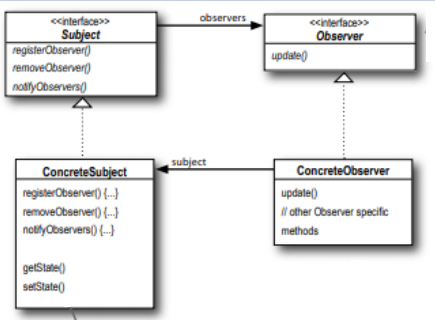
\includegraphics[width=7cm, height=6cm]{imagenes/observer.png}
\\
\item  \textbf{Ventajas}
\\-Permite  variar los sujetos y observadores indepedientemente.Se puede
rehusar sujetos  sin el rehuso de observadores  y viceversa.
\\-Permite agregar observadores sin modificar el sujeto o los observadores.
\item  \textbf{Desventajas}
\\-No se especifica  el receptor de una actualizacion.Se envia a todos los objetos interesados.
\\-Actualizaciones inesperadas.Se podrian dar actualizaciones en casacada muy ineficientes.

\item  \textbf{Ejemplo}
\\Crearemos un ejemplo en el cual al ingresar un monto en soles el programa
 nos dara la alerta segun el observador de cuando sera el cambio a la moneda de 
 ese observador.

\end{itemize}



 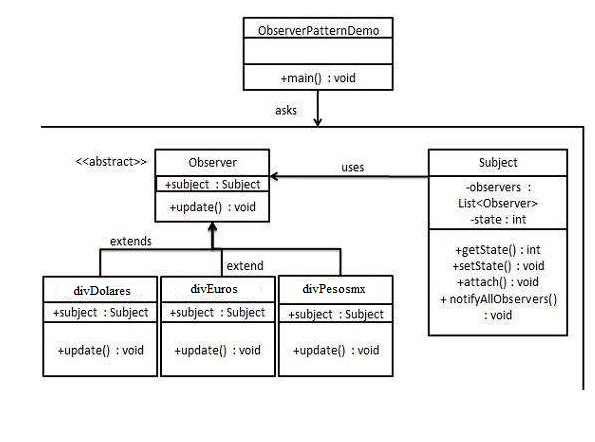
\includegraphics[width=7cm, height=7cm]{imagenes/observerEj.png}


\subsection{Segundo patron}


\begin{itemize}
\item subtitulo
\\ Contenido......
\\sub sub tiutl consalto de linea
\\LLenar completar......
\\ \textbf{- Para enumerar y resaltar}
\end{itemize}

\subsection{Tercer patron}
agregar
\subsection{Cuarto patron}
\subsection{Quinto patron}
\subsection{Sexto patron}
\subsection{Setimo patron}
\subsection{Octavo patron}



\section{Conclusiones}


\section{Recomendaciones}
%----------------------------------------------------------------------------------------
%	REFERENCE LIST
%----------------------------------------------------------------------------------------

\begin{thebibliography}{99} % Bibliography - this is intentionally simple in this template

\bibitem
Elisabeth Freeman, Kathy Sierra (2004).
\newblock Head First design patterns,
\newblock Sebastopol,
\newblock CA: O'Reilly.
 
 
\end{thebibliography}

%----------------------------------------------------------------------------------------

\end{document}